\section{Related Work}

\subsection{Music Theory Applications}
A search online and of the Apple ``App Store'' revealed several examples of applications which teach music theory, however none of these focus on writing music and are more based around ideas like flashcards and memorisation.

\begin{figure}[h!]
  \centering
  \frame{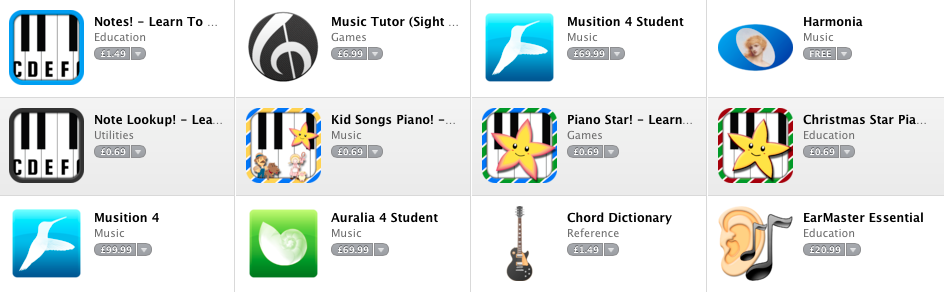
\includegraphics[width=\linewidth]{gfx/music-theory-apps.png}}
  \caption{Music Theory Applications after searching ``Music Theory'' on the Apple App Store}
\end{figure}

Most of these apps however, are aimed at more advanced students and miss out a huge part of theory exams which is the written notation section.

\subsection{Music Theory Workbooks}

\subsection{Existing OMR Applications}

Prior to embarking on a solution from scratch, an understanding of the existing OMR landscape and whether any tools already existed was done. Several software solutions were found which can help someone take a printed score (or even an older handwritten one) and process it to create a digital representation. However, the majority were commercial applications which required purchasing and almost were designed to be used under highly supervised conditions, doing an initial conversion and then guiding the user through the process of validating the applications `best guess'.

\begin{table}[h]
\caption{Comparison of existing OMR applications}
\begin{tabularx}{\linewidth}{ r | X }
    \textbf{Neuratron Photoscore}\footnote{http://www.neuratron.com/photoscore.htm} & One of the market leading packages, features tight integration with several composition tools like Sibelius and Finale, outputs to a range of formats (MusicXML etc). Designed to be run by the end user in supervised conditions, going over a scanned sheet and correcting errors as you go \\

    \ & \ \\
    \hline
    \ & \ \\

    \textbf{Audiveris}\footnote{https://audiveris.kenai.com/} & ``Audiveris is an open-source Optical Music Recognition software which processes the image of a music sheet to automatically provide symbolic music information in MusicXML standard.''\footnote{From the Audiveris website} \newline \newline At present it only supports high quality printed scores and operates by utilising a neural network which must be trained on samples by the end user. \\

    \ & \ \\
    \hline
    \ & \ \\

    \textbf{Gamera}\footnote{http://gamera.informatik.hsnr.de} & Gamera is primarily a structured document processing and symbol recognition tool \parencite{macmillan2002gamera} and was spun out of one of the authors' previous thesis which focussed on OMR \parencite{fujinaga1996adaptive}. Primarily used for academic purposes, it has some great projects, one of which specialises in supporting research into stave detection and removal \footnote{http://gamera.informatik.hsnr.de/addons/musicstaves/}. \\

    \ & \ \\
    \hline
    \ & \ \\

    \textbf{Capella Scan}\footnote{http://www.capella.de/us/index.cfm/products/capella-scan/info-capella-scan/} & As with most of the other applications mentioned, Capella scan is primarily designed to convert old or dated music manuscripts into a more ``preservable'' digital format without needing to manually type all the music out again. \\

\end{tabularx}
\end{table}
